% diagram_diffusion_process.png
% Training (one straight line) and generation (Euler steps) of a rectified flow model.
% Canvas: 15.23 cm x 5.00 cm (= \textwidth of the deck, height <= 5.0 cm).
\documentclass[border=0pt,11pt]{standalone}
\usepackage[T1]{fontenc}
\usepackage{lmodern}
\renewcommand{\familydefault}{\sfdefault}
\usepackage{tikz}
\usetikzlibrary{positioning,arrows.meta}

\definecolor{primaryNavy}{RGB}{24,24,27}
\definecolor{secondaryNavy}{RGB}{63,63,70}
\definecolor{mutedGray}{RGB}{248,250,252}
\definecolor{ruleGray}{RGB}{226,232,240}

\tikzset{
  box/.style={draw=secondaryNavy, line width=0.6pt, fill=mutedGray, rectangle,
              inner xsep=5pt, inner ysep=2.5pt, align=center,
              text=primaryNavy, font=\small},
  ar/.style={draw=secondaryNavy, line width=0.6pt,
             -{Latex[length=1.4mm,width=1.0mm]}},
  ret/.style={draw=secondaryNavy, line width=0.6pt, dashed,
              -{Latex[length=1.4mm,width=1.0mm]}},
  note/.style={text=primaryNavy, font=\footnotesize, fill=white,
               inner sep=1.5pt, align=center},
  rowlab/.style={text=primaryNavy, font=\small, align=center},
}

\begin{document}
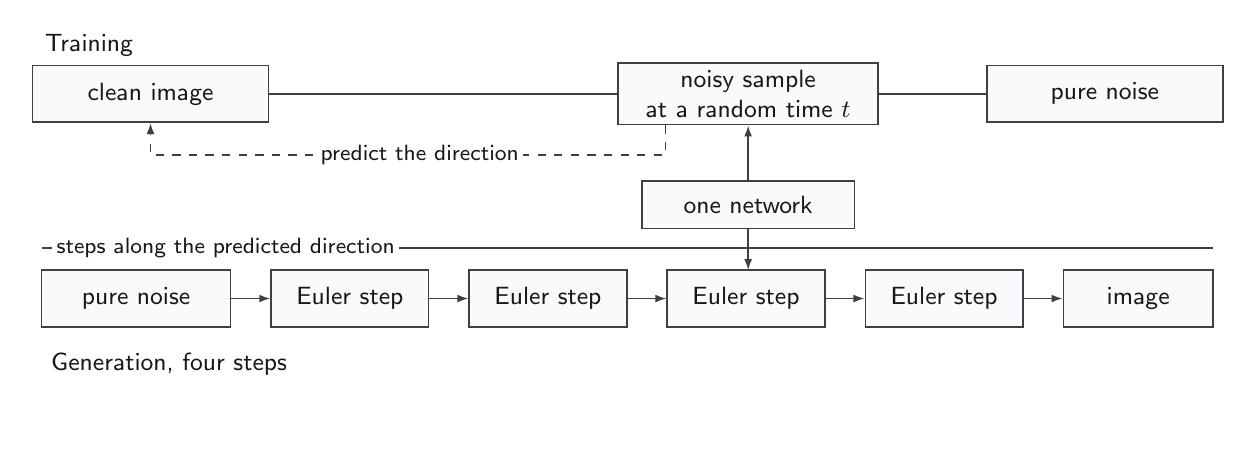
\begin{tikzpicture}[x=1cm,y=1cm]
\useasboundingbox (0,0) rectangle (15.23,5.00);
\fill[white] (0,0) rectangle (15.23,5.00);

% ---------------- top row: training ----------------
% One straight line between the clean image and pure noise; the sample in the
% middle is the mix at one random time, not a chain of noising steps.
\draw[draw=secondaryNavy, line width=0.6pt] (3.06,4.16) -- (12.18,4.16);
\node[box, minimum width=3.00cm, minimum height=0.72cm] (clean) at (1.56,4.16) {clean image};
\node[box, minimum width=3.30cm, minimum height=0.72cm] (sample) at (9.15,4.16) {noisy sample\\at a random time $t$};
\node[box, minimum width=3.00cm, minimum height=0.72cm] (pure)  at (13.68,4.16) {pure noise};

\node[rowlab] at (0.7797,4.78) {Training};

% the direction the model learns to predict: from the noisy sample to the image
\draw[ret] (8.10,0 |- sample.south) -- (8.10,3.38) -- (1.56,3.38) -- (clean.south);
\node[note] at (4.98,3.38) {predict the direction};

% ---------------- shared network box ----------------
\node[box, minimum width=2.70cm, minimum height=0.60cm] (net) at (9.15,2.75) {one network};
\draw[ar] (net.north) -- (sample.south);
\draw[ar] (net.south) -- (9.15,1.92);

% ---------------- bottom row: generation ----------------
\node[box, minimum width=2.40cm, minimum height=0.72cm] (gnoise) at (1.3764,1.56) {pure noise};
\node[box, minimum width=2.00cm, minimum height=0.72cm] (d1) at (4.0918,1.56) {Euler step};
\node[box, minimum width=2.00cm, minimum height=0.72cm] (d2) at (6.6073,1.56) {Euler step};
\node[box, minimum width=2.00cm, minimum height=0.72cm] (d3) at (9.1227,1.56) {Euler step};
\node[box, minimum width=2.00cm, minimum height=0.72cm] (d4) at (11.6382,1.56) {Euler step};
\node[box, minimum width=1.90cm, minimum height=0.72cm] (img) at (14.1036,1.56) {image};

\draw[ar] (gnoise.east) -- (d1.west);
\draw[ar] (d1.east) -- (d2.west);
\draw[ar] (d2.east) -- (d3.west);
\draw[ar] (d3.east) -- (d4.west);
\draw[ar] (d4.east) -- (img.west);

% direction annotation above the generation row
\draw[draw=secondaryNavy, line width=0.6pt] (0.1764,2.20) -- (15.0536,2.20);
\node[note] at (2.5136,2.20) {steps along the predicted direction};

\node[rowlab] at (1.7957,0.72) {Generation, four steps};

\end{tikzpicture}
\end{document}
